\documentclass[color=usenames,dvipsnames]{beamer}\usepackage[]{graphicx}\usepackage[]{color}
% maxwidth is the original width if it is less than linewidth
% otherwise use linewidth (to make sure the graphics do not exceed the margin)
\makeatletter
\def\maxwidth{ %
  \ifdim\Gin@nat@width>\linewidth
    \linewidth
  \else
    \Gin@nat@width
  \fi
}
\makeatother

\definecolor{fgcolor}{rgb}{0.345, 0.345, 0.345}
\newcommand{\hlnum}[1]{\textcolor[rgb]{0.686,0.059,0.569}{#1}}%
\newcommand{\hlstr}[1]{\textcolor[rgb]{0.192,0.494,0.8}{#1}}%
\newcommand{\hlcom}[1]{\textcolor[rgb]{0.678,0.584,0.686}{\textit{#1}}}%
\newcommand{\hlopt}[1]{\textcolor[rgb]{0,0,0}{#1}}%
\newcommand{\hlstd}[1]{\textcolor[rgb]{0.345,0.345,0.345}{#1}}%
\newcommand{\hlkwa}[1]{\textcolor[rgb]{0.161,0.373,0.58}{\textbf{#1}}}%
\newcommand{\hlkwb}[1]{\textcolor[rgb]{0.69,0.353,0.396}{#1}}%
\newcommand{\hlkwc}[1]{\textcolor[rgb]{0.333,0.667,0.333}{#1}}%
\newcommand{\hlkwd}[1]{\textcolor[rgb]{0.737,0.353,0.396}{\textbf{#1}}}%
\let\hlipl\hlkwb

\usepackage{framed}
\makeatletter
\newenvironment{kframe}{%
 \def\at@end@of@kframe{}%
 \ifinner\ifhmode%
  \def\at@end@of@kframe{\end{minipage}}%
  \begin{minipage}{\columnwidth}%
 \fi\fi%
 \def\FrameCommand##1{\hskip\@totalleftmargin \hskip-\fboxsep
 \colorbox{shadecolor}{##1}\hskip-\fboxsep
     % There is no \\@totalrightmargin, so:
     \hskip-\linewidth \hskip-\@totalleftmargin \hskip\columnwidth}%
 \MakeFramed {\advance\hsize-\width
   \@totalleftmargin\z@ \linewidth\hsize
   \@setminipage}}%
 {\par\unskip\endMakeFramed%
 \at@end@of@kframe}
\makeatother

\definecolor{shadecolor}{rgb}{.97, .97, .97}
\definecolor{messagecolor}{rgb}{0, 0, 0}
\definecolor{warningcolor}{rgb}{1, 0, 1}
\definecolor{errorcolor}{rgb}{1, 0, 0}
\newenvironment{knitrout}{}{} % an empty environment to be redefined in TeX

\usepackage{alltt}
%\documentclass[color=usenames,dvipsnames,handout]{beamer}

%\usepackage[roman]{../pres1}
\usepackage[sans]{../pres1}
\usepackage{graphicx}
\usepackage{bm}
%\usepackage{changepage}

%\newcommand{\wide}{\column{\dimexpr\paperwidth}} % Must be in columns environment




\IfFileExists{upquote.sty}{\usepackage{upquote}}{}
\begin{document}


\begin{frame}[plain]
  \begin{center}
    {\huge Stochasticity} \\
%    { February 4, 2019} \\
    \vfill
    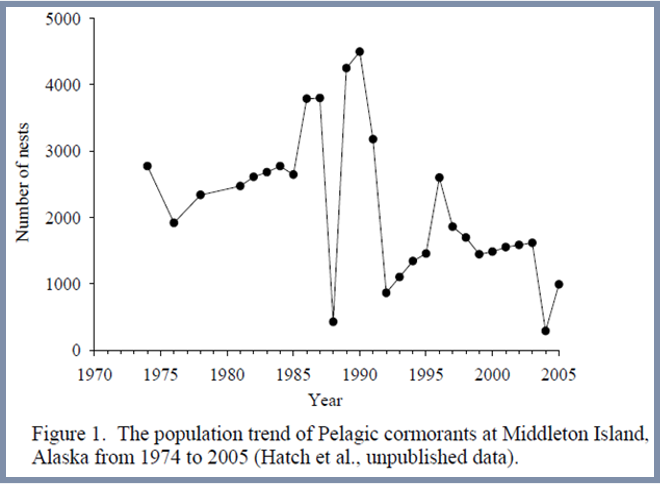
\includegraphics[height=3.8cm,keepaspectratio]{figs/pelagic-cormorants} \hspace{0.1cm}
    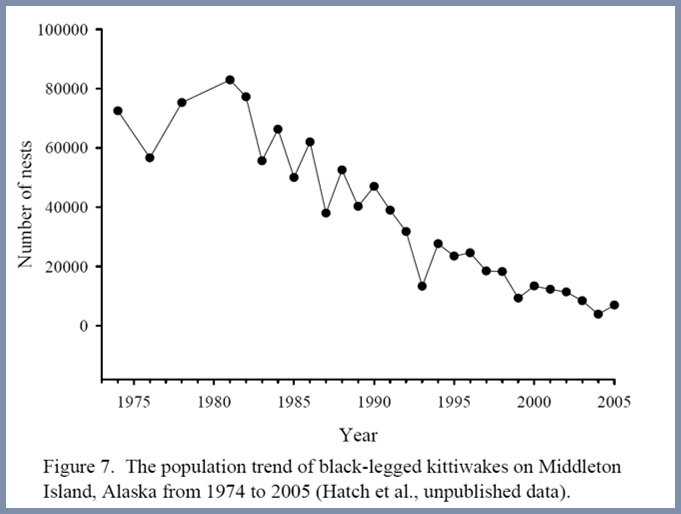
\includegraphics[height=3.8cm,keepaspectratio]{figs/kittiwakes} %\hspace{0.5cm}
%    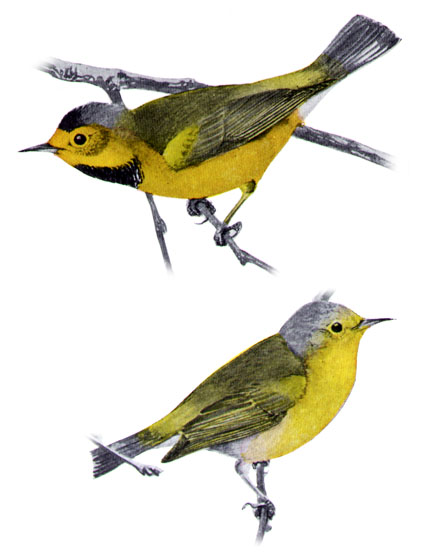
\includegraphics[height=5.5cm,keepaspectratio]{figs/Vermivora_bachmanii} %\hspace{0.1cm}
  \end{center}
\end{frame}




\section{Introduction}


\begin{frame}[plain]
  \frametitle{Today's topics}
  \tableofcontents%[currentsection]
\end{frame}




\begin{frame}
  \frametitle{Random Variables}
  \large
  A random variable is a variable whose value can't be predicted
  with certainty. \\
  \pause
  \vfill
  Examples?
  \begin{itemize}
    \item Weather
    \item Our own behavior
    \item Population size
  \end{itemize}
\end{frame}




\begin{frame}
  \frametitle{Probability distributions}
  \large
  {A random variable ($X$) can be described by a probability distribution. \\}
  \pause
  \vspace{1cm}
  {There are many types of probability distributions}
  \begin{itemize}
    \item Normal (or Gaussian)
    \item Poisson
    \item Binomial
    \item Multinomial
    \item etc\dots
  \end{itemize}
\end{frame}





\begin{frame}[fragile]
  \frametitle{Normal (Gaussian) Distribution}
\[
  X \sim \mbox{Normal}(\mu=0, \sigma^2=1)
\]

\vspace{-1cm}
%\centering
\begin{center}
  \includegraphics<1 | handout:0>[width=\textwidth]{figs/norm/norm0} %\\
  \includegraphics<2 | handout:0>[width=\textwidth]{figs/norm/norm1} %\\
  \includegraphics<3 | handout:0>[width=\textwidth]{figs/norm/norm2} %\\
  \includegraphics<4 | handout:0>[width=\textwidth]{figs/norm/norm3} %\\
  \includegraphics<5 | handout:0>[width=\textwidth]{figs/norm/norm4} %\\
  \includegraphics<6 | handout:0>[width=\textwidth]{figs/norm/norm5} %\\
  \includegraphics<7 | handout:0>[width=\textwidth]{figs/norm/norm6} %\\
  \includegraphics<8 | handout:0>[width=\textwidth]{figs/norm/norm7} %\\
  \includegraphics<9 | handout:0>[width=\textwidth]{figs/norm/norm8} %\\
  \includegraphics<10 | handout:0>[width=\textwidth]{figs/norm/norm9} %\\
  \includegraphics<11->[width=\textwidth]{figs/norm/norm10} %\\
\end{center}

\end{frame}






\begin{frame}[fragile]
  \frametitle{Normal (Gaussian) Distribution}
  \vspace{-0.7cm}
  \begin{center}

  \end{center}
\includegraphics[width=\textwidth]{figure/norm1-1}
\end{frame}





\begin{frame}[fragile]
  \frametitle{A purely stochastic model}
  \vspace{-3mm}
  \[
    N_t \sim \mbox{Normal}(\mu=50, \sigma^2=1)
  \]
  \vspace{-8mm}

\begin{center}
%  \includegraphics[width=0.7\textwidth]{stochasticity-normpop}
  \includegraphics[width=0.9\textwidth]{figure/normpop-1}
\end{center}
\note{Amazing that this looks more realistic than a theoretical model}
\end{frame}



\begin{frame}
  \frametitle{Two important types of stochasticity}
  {\bf Environmental stochasticity}
  \begin{itemize}
    \item Random variation in weather, habitat, etc\dots among years
    \item[]
  \end{itemize}
  \pause
  {\bf Demographic stochasticity}
  \begin{itemize}
    \item Random variation in the number of births and deaths among years
    \item[]
  \end{itemize}
\end{frame}







\section{Geometric Growth}





\begin{frame}[fragile]
  \frametitle{Geometric growth with environmental stochasticity}
  \Large
\[
  N_{t+1} = N_t + N_tr + X_t
\]
%\vspace{0.3cm} \pause
{\large \centering where \\}
\[
  X_t \sim \mbox{Normal}(0, \sigma_e^2)
\]
\pause
\vfill
{\tt \R} code:
\begin{knitrout}\small
\definecolor{shadecolor}{rgb}{0.969, 0.969, 0.969}\color{fgcolor}\begin{kframe}
\begin{alltt}
\hlstd{r} \hlkwb{<-} \hlnum{0.1}
\hlstd{sigma.e} \hlkwb{<-} \hlnum{10}
\hlkwa{for}\hlstd{(t} \hlkwa{in} \hlnum{2}\hlopt{:}\hlstd{nYears) \{}
    \hlstd{X[t}\hlopt{-}\hlnum{1}\hlstd{]} \hlkwb{<-} \hlkwd{rnorm}\hlstd{(}\hlkwc{n}\hlstd{=}\hlnum{1}\hlstd{,} \hlkwc{mean}\hlstd{=}\hlnum{0}\hlstd{,} \hlkwc{sd}\hlstd{=sigma.e)}
    \hlstd{N[t]} \hlkwb{<-} \hlstd{N[t}\hlopt{-}\hlnum{1}\hlstd{]} \hlopt{+} \hlstd{N[t}\hlopt{-}\hlnum{1}\hlstd{]}\hlopt{*}\hlstd{r} \hlopt{+} \hlstd{X[t}\hlopt{-}\hlnum{1}\hlstd{]}
\hlstd{\}}
\end{alltt}
\end{kframe}
\end{knitrout}
\end{frame}






\begin{frame}[fragile]
  \frametitle{Example $N_0=100$, $r=0.1$, $\mu=0$, $\sigma_e^2=100$}

\vspace{-0.1cm}
\begin{center}
  \includegraphics<1 | handout:0>[width=\textwidth]{figs/exp-e/exp-e1}
  \includegraphics<2 | handout:0>[width=\textwidth]{figs/exp-e/exp-e2}
  \includegraphics<3 | handout:0>[width=\textwidth]{figs/exp-e/exp-e3}
  \includegraphics<4 | handout:0>[width=\textwidth]{figs/exp-e/exp-e4}
  \includegraphics<5 | handout:0>[width=\textwidth]{figs/exp-e/exp-e5}
  \includegraphics<6 | handout:0>[width=\textwidth]{figs/exp-e/exp-e6}
  \includegraphics<7 | handout:0>[width=\textwidth]{figs/exp-e/exp-e7}
  \includegraphics<8 | handout:0>[width=\textwidth]{figs/exp-e/exp-e8}
  \includegraphics<9 | handout:0>[width=\textwidth]{figs/exp-e/exp-e9}
  \includegraphics<10>[width=\textwidth]{figs/exp-e/exp-e10}
\end{center}
\end{frame}





\begin{frame}[fragile]
  \frametitle{Example $N_0=100$, $r=0.1$, $\mu=0$, $\sigma_e^2=10000$}

\vspace{-0.1cm}
\begin{center}
  \includegraphics<1 | handout:0>[width=\textwidth]{figs/exp-e2/exp-e1}
  \includegraphics<2 | handout:0>[width=\textwidth]{figs/exp-e2/exp-e2}
  \includegraphics<3 | handout:0>[width=\textwidth]{figs/exp-e2/exp-e3}
  \includegraphics<4 | handout:0>[width=\textwidth]{figs/exp-e2/exp-e4}
  \includegraphics<5 | handout:0>[width=\textwidth]{figs/exp-e2/exp-e5}
  \includegraphics<6 | handout:0>[width=\textwidth]{figs/exp-e2/exp-e6}
  \includegraphics<7 | handout:0>[width=\textwidth]{figs/exp-e2/exp-e7}
  \includegraphics<8 | handout:0>[width=\textwidth]{figs/exp-e2/exp-e8}
  \includegraphics<9 | handout:0>[width=\textwidth]{figs/exp-e2/exp-e9}
  \includegraphics<10>[width=\textwidth]{figs/exp-e2/exp-e10}
\end{center}
\end{frame}







\begin{frame}
  \frametitle{Geometric growth with demographic stochasticity}
  \LARGE
\[
  N_{t+1} = N_t + N_t r_t
\]

\vspace{0.3cm} \pause
{\large \centering where \par}
\[
  r_t \sim \mbox{Normal}(\bar{r}, \sigma_d^2)
\]
\end{frame}









\begin{frame}[fragile]
  \frametitle{Example $N_0=100$, $\bar{r}=0.5$, $\sigma_d^2=0.01$}

\vspace{-0.3cm}
\begin{center}
  \includegraphics<1 | handout:0>[width=\textwidth]{figs/exp-d/exp-d1}
  \includegraphics<2 | handout:0>[width=\textwidth]{figs/exp-d/exp-d2}
  \includegraphics<3 | handout:0>[width=\textwidth]{figs/exp-d/exp-d3}
  \includegraphics<4 | handout:0>[width=\textwidth]{figs/exp-d/exp-d4}
  \includegraphics<5 | handout:0>[width=\textwidth]{figs/exp-d/exp-d5}
  \includegraphics<6 | handout:0>[width=\textwidth]{figs/exp-d/exp-d6}
  \includegraphics<7 | handout:0>[width=\textwidth]{figs/exp-d/exp-d7}
  \includegraphics<8 | handout:0>[width=\textwidth]{figs/exp-d/exp-d8}
  \includegraphics<9 | handout:0>[width=\textwidth]{figs/exp-d/exp-d9}
  \includegraphics<10>[width=\textwidth]{figs/exp-d/exp-d10}
\end{center}
\end{frame}






\begin{frame}[fragile]
  \frametitle{Example $N_0=100$, $\bar{r}=0.5$, $\sigma_d^2=0.25$}

\vspace{-0.3cm}
\begin{center}
  \includegraphics<1 | handout:0>[width=\textwidth]{figs/exp-d2/exp-d1}
  \includegraphics<2 | handout:0>[width=\textwidth]{figs/exp-d2/exp-d2}
  \includegraphics<3 | handout:0>[width=\textwidth]{figs/exp-d2/exp-d3}
  \includegraphics<4 | handout:0>[width=\textwidth]{figs/exp-d2/exp-d4}
  \includegraphics<5 | handout:0>[width=\textwidth]{figs/exp-d2/exp-d5}
  \includegraphics<6 | handout:0>[width=\textwidth]{figs/exp-d2/exp-d6}
  \includegraphics<7 | handout:0>[width=\textwidth]{figs/exp-d2/exp-d7}
  \includegraphics<8 | handout:0>[width=\textwidth]{figs/exp-d2/exp-d8}
  \includegraphics<9 | handout:0>[width=\textwidth]{figs/exp-d2/exp-d9}
  \includegraphics<10>[width=\textwidth]{figs/exp-d2/exp-d10}
\end{center}
\end{frame}





\section{Logistic growth}




\begin{frame}
  \frametitle{Logistic growth with stochastic carrying capacity}
  \LARGE
\[
  N_{t+1} = N_t + N_tr_{max}(1 - N_t/K_t)
\]

\vspace{0.3cm}
{\large \centering where \par}
\[
  K_t \sim \mbox{Normal}(\bar{K}, \sigma_e^2)
\]
\end{frame}






\begin{frame}[fragile]
  \frametitle{Logistic example, $r_{max}=0.2$, $\bar{K}=100$, $\sigma_e^2=400$}

\vspace{-0.2cm}
\begin{center}
  \includegraphics<1 | handout:0>[width=\textwidth]{figs/lg-d/lg-d1}
  \includegraphics<2 | handout:0>[width=\textwidth]{figs/lg-d/lg-d2}
  \includegraphics<3 | handout:0>[width=\textwidth]{figs/lg-d/lg-d3}
  \includegraphics<4 | handout:0>[width=\textwidth]{figs/lg-d/lg-d4}
  \includegraphics<5 | handout:0>[width=\textwidth]{figs/lg-d/lg-d5}
  \includegraphics<6 | handout:0>[width=\textwidth]{figs/lg-d/lg-d6}
  \includegraphics<7 | handout:0>[width=\textwidth]{figs/lg-d/lg-d7}
  \includegraphics<8 | handout:0>[width=\textwidth]{figs/lg-d/lg-d8}
  \includegraphics<9 | handout:0>[width=\textwidth]{figs/lg-d/lg-d9}
  \includegraphics<10>[width=\textwidth]{figs/lg-d/lg-d10}
\end{center}
\end{frame}



\begin{frame}
  \frametitle{Summary}
  \Large
%  \begin{itemize}[<+->]
%    \item Stochasticity is everywhere and we have to recognize it our models
%    \item Stochastic models produce outcomes that look like real data
%    \item
  Purely deterministic models are too rigid \\
  \vfill
  % \item
  Purely stochastic models don't tell us much \\
  \vfill
  % \item
  The goal is to develop a mechanistic model that represents 
  our biological understanding while allowing for stochasticity \\
%  \end{itemize}
\end{frame}


%\begin{frame}
%  \frametitle{Assignment}
%  \Large
%   Read pages 19--22 in Conroy and Carroll
%\end{frame}







% quasi-equilibrium



%% \subsection{Birth-death process}


%% \begin{frame}
%%   \frametitle{Birth-death process}
%%   What does it mean for $r$ to be random?
%% \end{frame}


\end{document}


